\documentclass[letterpaper,spanish,reprint,nofootinbib,showkeys,aps]{revtex4-2}

%%%%%%%%%%%%%%%%%%%%%%%%%%%%%%%%%%%%%%%%%%%%%%%%%%%%%%%%%%%%%%%%%%%%%%%%%%%%
% PAQUETES USUALES
\usepackage[T1]{fontenc}
\usepackage[utf8]{inputenc}
\usepackage[spanish]{babel} 
\usepackage{calc}
\usepackage{amsmath,bm,amssymb}
\usepackage{fancyhdr}
\usepackage{pythonhighlight}
\usepackage{graphicx}
\usepackage{float}\usepackage{xcolor}
%para escribir código%%%%%%%%%%%%%%
\usepackage{algorithm}
\usepackage{algpseudocode}
\usepackage{listings}
\usepackage{color, xcolor}
%\usepackage[backend=biber]{biblatex}
%%%Algunos comandos útiles para el PDF generado%%%
\usepackage[unicode=true,pdfusetitle, bookmarks=true,bookmarksnumbered=false,bookmarksopen=false, breaklinks=false,pdfborder={0 0 1},backref=false,colorlinks=true] {hyperref}
\hypersetup{
 citecolor=dkgreen,linkcolor=blue,urlcolor=blue}
%%% PARA TEOREMAS NUEVOS
\usepackage{amsthm}
\renewcommand{\qedsymbol}{\tiny{$\blacksquare$}}
\newenvironment{solucion}{\begin{proof}[\textcolor{magenta}{Solución}]}{\end{proof}}
\usepackage{mdframed}
\usepackage[many]{tcolorbox}
\usepackage{thmtools}


%%%%%%%%%%%%%%%%%%%%%%%%%%%%%%%%%%%%%%%%%%%%%%%%%%%%%%%%%%%%%%%%%%%%%%%%%%%%
%%%%%%%%%%%%%%%%%%%%%%%%%%%%%%%%%%%%%%%%%%%%%%%%%%%%%%%%%%%%%%%%%%%%%%%%%%%%
%%%%%%%%%%%%%%%%%%%%%%%%%%%% MARGENES %%%%%%%%%%%%%%%%%%%%%%%%%%%%%%%%%%%%%%
%%%%%%%%%%%%%%%%%%%%%%%%%%%%%%%%%%%%%%%%%%%%%%%%%%%%%%%%%%%%%%%%%%%%%%%%%%%%
%%%%%%%%%%%%%%%%%%%%%%%%%%%%%%%%%%%%%%%%%%%%%%%%%%%%%%%%%%%%%%%%%%%%%%%%%%%%

\parskip=5pt
\hoffset = 0pt
\headsep = 0.8 cm % estaba en 1.5 cm, lo cambie para el header de la imagen
\setlength{\parindent}{0cm}

%%%%%%%%%%%%%%%%%%%%%%%%%%%%%%%%%%%%%%%%%%%%%%%%%%%%%%%%%%%%%%%%%%%%%%%%%%%%
%%%%%%%%%%%%%%%%%%%%%%%%%%%%%%%%%%%%%%%%%%%%%%%%%%%%%%%%%%%%%%%%%%%%%%%%%%%%
%%%%%%%%%%%%%%%%%%%%%%%%% EJERRCICIOS  %%%%%%%%%%%%%%%%%%%%%%%%%%%%%%%%%%%%%
%%%%%%%%%%%%%%%%%%%%%%%%%%%%%%%%%%%%%%%%%%%%%%%%%%%%%%%%%%%%%%%%%%%%%%%%%%%%
%%%%%%%%%%%%%%%%%%%%%%%%%%%%%%%%%%%%%%%%%%%%%%%%%%%%%%%%%%%%%%%%%%%%%%%%%%%%

\newtcolorbox[auto counter,number within=section]{ejercicio}[1][]{
% ESTO ES PARA LA CAJA GENERAL
breakable, % por si cambias de pagina
enhanced, % estilo general
% TITULO MODIFICACIONES
coltitle= black,
colbacktitle= white,
titlerule= 0mm,
colframe = magenta,
fonttitle=\bfseries,
title= Ejercicio~\thetcbcounter,
% CAJA LINEA MODIFICACIONES
boxed title style={
  sharp corners,
  rounded corners=northwest,
  rounded corners=northeast,
  % outer arc=0pt,
  % arc=0pt,
  },
% CONTENIDO MODIFICACIONES
colback = white,
fontupper = \itshape,
coltext =  black,
% MARCO MODIFICACIONES
rightrule=0mm,
toprule=0pt,
bottomrule= 0pt,
leftrule = 4pt
}

%%%%%%%%%%%%%%%%%%%%%%%%%%%%%%%%%%%%%%%%%%%%%%%%%%%%%%%%%%%%%%%%%%%%%%%%%%%%
%%%%%%%%%%%%%%%%%%%%%%%%%%%%%%%%%%%%%%%%%%%%%%%%%%%%%%%%%%%%%%%%%%%%%%%%%%%%
%%%%%%%%%%%%%%%%%%%%%%%%% PYTHON Y C %%%%%%%%%%%%%%%%%%%%%%%%%%%%%%%%%%
%%%%%%%%%%%%%%%%%%%%%%%%%%%%%%%%%%%%%%%%%%%%%%%%%%%%%%%%%%%%%%%%%%%%%%%%%%%%
%%%%%%%%%%%%%%%%%%%%%%%%%%%%%%%%%%%%%%%%%%%%%%%%%%%%%%%%%%%%%%%%%%%%%%%%%%%%


\definecolor{dkgreen}{rgb}{0.9,0.6,0.8}
\definecolor{blue}{rgb}{0.0,0.49,0.4}
\definecolor{gray97}{gray}{.97}
\definecolor{gray75}{gray}{.75}
\definecolor{gray45}{gray}{.45}
\definecolor{codegreen}{rgb}{0,0.6,0}
\definecolor{codegray}{rgb}{0.5,0.5,0.5}
\definecolor{codepurple}{rgb}{0.58,0,0.82}
\definecolor{backcolour}{rgb}{0.95,0.95,0.92}

\lstdefinestyle{mystyle}{
    backgroundcolor=\color{gray97},
    commentstyle=\color{cyan!75!black},
    keywordstyle=\color{magenta},
    numberstyle=\tiny\color{codegray},
    stringstyle=\color{codepurple},
    basicstyle=\ttfamily\footnotesize,
    breakatwhitespace=false,
    breaklines= true,
    captionpos=b,
    keepspaces=true,
    numbers=left,
    numbersep=5pt,
    showspaces=false,
    showstringspaces=false,
    showtabs=false,
    tabsize=2,
    language=bash,   %% PHP, C, Java, etc... bash is the standard
    extendedchars=true,
    inputencoding=latin1
}

\lstset{style=mystyle, literate =
                        {í}{{\'i}}1
                        {á}{{\'a}}1
                        {é}{{\'e}}1
                        {ó}{{\'o}}1
                        {ú}{{\'u}}1
                        {ñ}{{\~n}}1
                        {ü}{{\"u}}1
                            }

%%%%%%%%%%%%%%%%%%%%%%%%%%%%%%%%%%%%%%%%%%%%%%%%%%%%%%%%%%%%%%%%%%%%%%%%%%%%
%%%%%%%%%%%%%%%%%%%%%%%%%%%%%%%%%%%%%%%%%%%%%%%%%%%%%%%%%%%%%%%%%%%%%%%%%%%%
%%%%%%%%%%%%%%%%%%%%% ##ENCABEZADOS Y NUMERACION %%%%%%%%%%%%%%%%%%%%%%%%%%%%%
%%%%%%%%%%%%%%%%%%%%%%%%%%%%%%%%%%%%%%%%%%%%%%%%%%%%%%%%%%%%%%%%%%%%%%%%%%%%
%%%%%%%%%%%%%%%%%%%%%%%%%%%%%%%%%%%%%%%%%%%%%%%%%%%%%%%%%%%%%%%%%%%%%%%%%%%%

\pagestyle{fancy}
\fancyhf{}
\fancyfoot{\thepage}
\fancyfoot[R]{\small{\textsc{Y. Sarahi García González}}}
\fancyfoot[L]{\small{\textsc{Proyecto tecnológicio de verano}}}
\chead{\includegraphics[scale=.27]{/Users/ely/Documents/Plantilla/Figures/waves.pdf}}
\renewcommand{\headrulewidth}{0pt}
\renewcommand{\footrulewidth}{0pt}

%%%%%%%%%%%%%%%%%%%%%%%%%%%%%%%%%%%%%%%%%%%%%%%%%%%%%%%%%%%%%%%%%%%%%%%%%%%%
%%%%%%%%%%%%%%%%%%%%%%%%%%%%%%%%%%%%%%%%%%%%%%%%%%%%%%%%%%%%%%%%%%%%%%%%%%%%
%%%%%%%%%%%%%%%%%%%%%%%%%%%%%%%%%%%%%%%%%%%%%%%%%%%%%%%%%%%%%%%%%%%%%%%%%%%%
%%%%%%%%%%%%%%%%%%%%%%%%%%%%%%%%%%%%%%%%%%%%%%%%%%%%%%%%%%%%%%%%%%%%%%%%%%%%

%%%Declaración de operadores%%%
\DeclareMathOperator{\sech}{sech}

%%%%%%%%%%%%%%%%%%%%%%%%%%%%%%%%%%%%%%%%%%%%%%%%%%%%%%%%%%%%%%%%%%%%%%%%%%%%
%%%%%%%%%%%%%%%%%%%%%%%%%%%%%%%%%%%%%%%%%%%%%%%%%%%%%%%%%%%%%%%%%%%%%%%%%%%%
%%%%%%%%%%%%%%%%%%%%%%%%%%%%%%%%%%%%%%%%%%%%%%%%%%%%%%%%%%%%%%%%%%%%%%%%%%%%
%%%%%%%%%%%%%%%%%%%%%%%%%%%%%%%%%%%%%%%%%%%%%%%%%%%%%%%%%%%%%%%%%%%%%%%%%%%%


\begin{document}

\preprint{NLP}
\title{\Large{\textbf{Natural Language Processing Applied to Bioinformatics}}}
%\thanks{A footnote to the article title}
\author{Y. Sarahi García González}
\email{yesenia.garcia@cimat.mx}
\affiliation{\vspace{0.15cm}Centro de Investigación en Matemáticas CIMAT}
\thanks{PLN a  cargo de Dr. J. Fernando Sánchez Vega}


%%%%%%%%%%%%%%%%%%%%%%%%%%%%%%%%%%%%%%%%%%%%%%%%%%%%%%%%%%%%%%%%%%%%%%%%%%%%
%%%%%%%%%%%%%%%%%%%%%%%%%%%%%%%%%%%%%%%%%%%%%%%%%%%%%#0Abstract%%%%%%%%%%%%%%%
%%%%%%%%%%%%%%%%%%%%%%%%%%%%%%%%%%%%%%%%%%%%%%%%%%%%%%%%%%%%%%%%%%%%%%%%%%%%
%%%%%%%%%%%%%%%%%%%%%%%%%%%%%%%%%%%%%%%%%%%%%%%%%%%%%%%%%%%%%%%%%%%%%%%%%%%%

\begin{abstract}
\begin{center}
\small{July, 2024}
\end{center}
\vspace{0.6cm}


In this work, we explore applying large language models for predicting protein solubility and fluorescence using only protein sequences datasets from the TorchDrug library. 
For solubility prediction, we employed a modified version of the PeptideBERT architecture. This model, configured with 12 hidden layers and 12 attention heads, was adjusted to handle sequences of up to 512 amino acids, achieving 67.98$\% $accuracy. In contrast, the ProtBERT model used in PEER was trained with longer sequences and a more robust configuration, achieving slightly higher accuracy.
In the fluorescence prediction task, we used a similar model based on PeptideBERT but modified for regression. The performance evaluation showed a test Spearman's rank correlation coefficient of 0.23, indicating a low performance. This result can be attributed to the dataset's nature, the model's inadequacy for this specific task, and the limited number of training epochs.

\end{abstract}

\maketitle

%%%%%%%%%%%%%%%%%%%%%%%%%%%%%%%%%%%%%%%%%%%%%%%%%%%%%%%%%%%%%%%%%%%%%%%%%%%%
%%%%%%%%%%%%%%%%%%%%%%%%%%%%%%%%%%%%%%%%%%%%%%%%%%%#1INTRODUCION%%%%%%%%%%%%%
%%%%%%%%%%%%%%%%%%%%%%%%%%%%%%%%%%%%%%%%%%%%%%%%%%%%%%%%%%%%%%%%%%%%%%%%%%%%



\section{Introduction}
%  qué es PEER, cuáles son las dos tareas a reproducir, importnacia de tareas: en qué áreas es importante conocer esas propiedades

%aplicaciones:predicción de estructura, diseño,predicción de propiedades.



Proteins are fundamental components of all living cells and play a critical role in many biological processes. They act as enzymes and structural elements essential for the structure, function, and regulation of the body's tissues and organs \cite{genomeglossary_protein} . They are also key players in the immune system. Antibodies are proteins that recognize and neutralize pathogens such as bacteria and viruses.\cite{hu2024survey} 


Every protein is made up of one or more chains of amino acids (called polypeptides)  that fold into complex ensembles of three-dimensional structures that determine its functions \cite{genomeglossary_protein}.  The DNA sequence of the protein-encoding gene determines these chains or sequences: mRNA is read and translated into the string of amino acid chains that make up the synthesized protein (this process is called translation). \cite{genomeglossary_translation} 


\begin{figure} [H]
	\begin{center}
		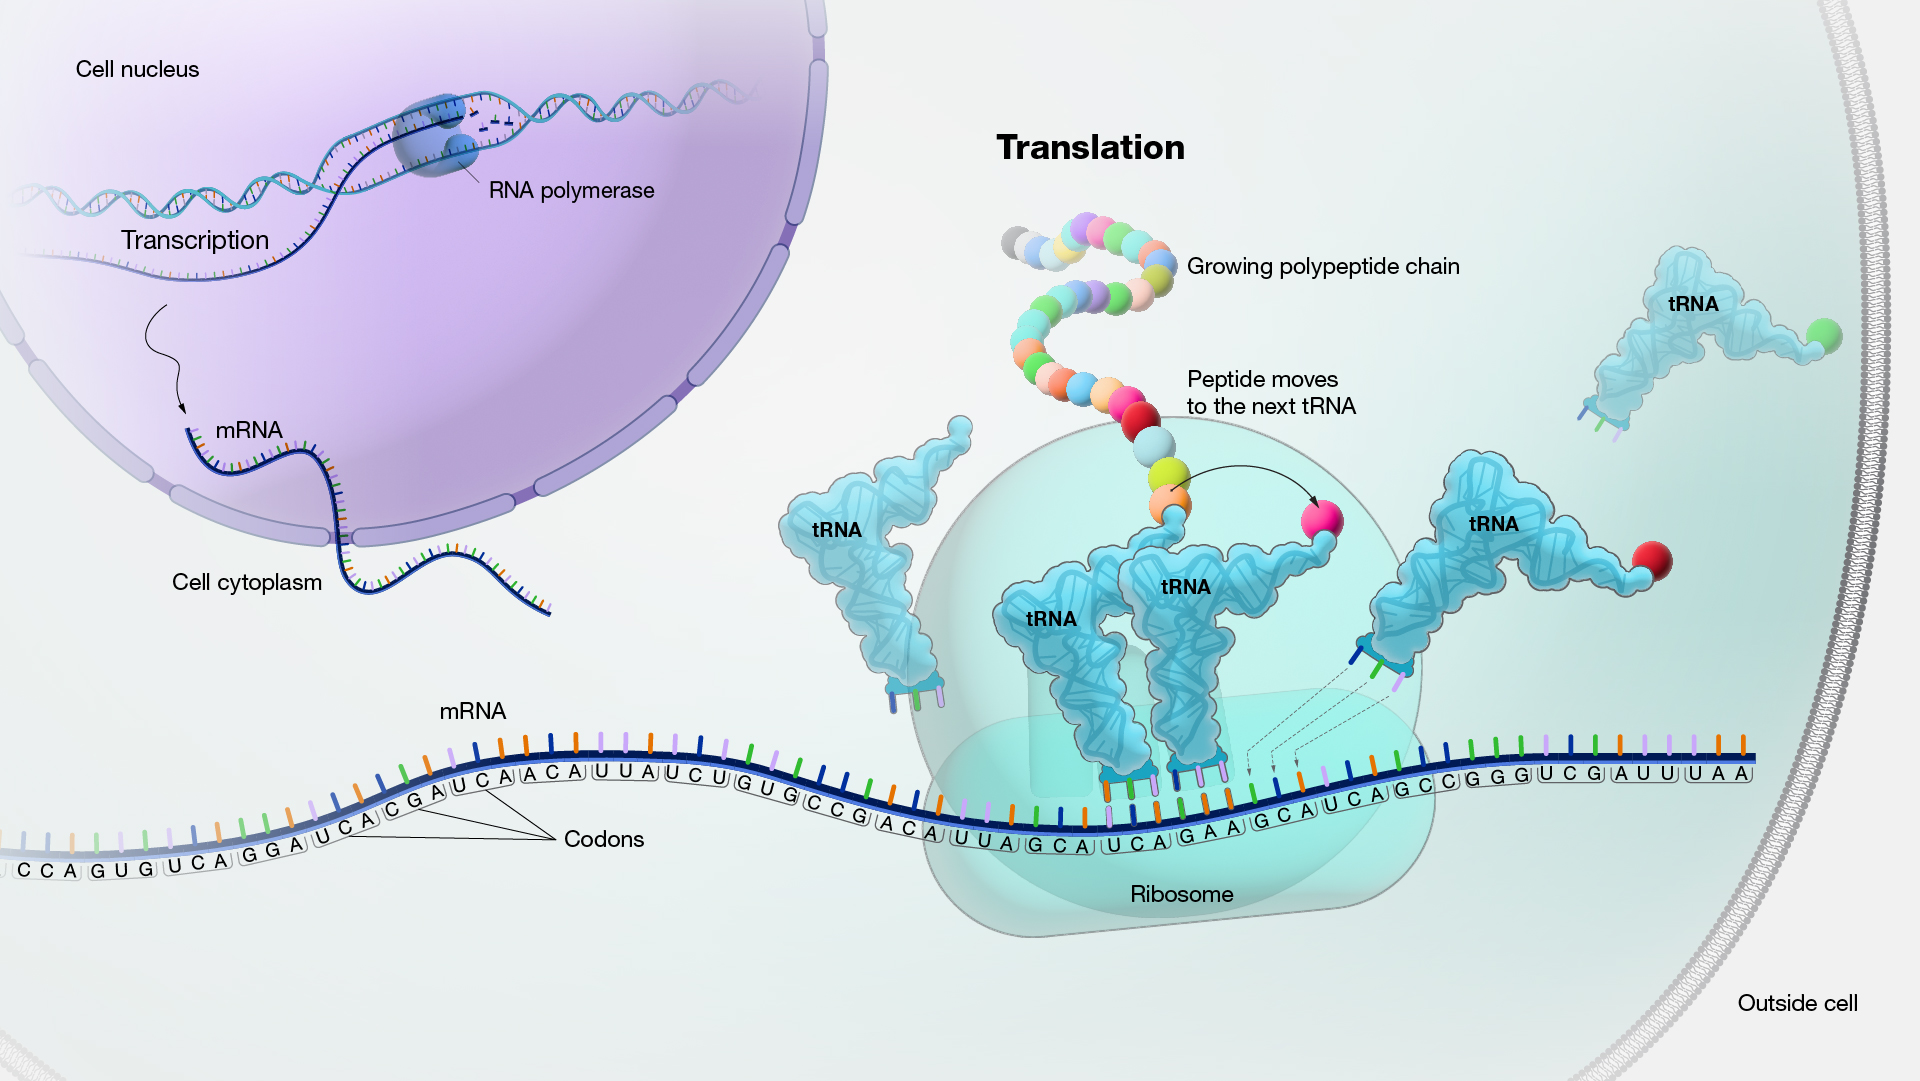
\includegraphics[scale=0.11]{/Users/ely/Documents/Maestria/proyecto_tecnologico/cimat2024-proyecto/Trabajo_final/latex/imagenes/Translation.jpg}
		\caption{Translation is the process through which information encoded in messenger RNA directs the addition of amino acids during protein synthesis. Translation occurs on ribosomes in the cell cytoplasm. \cite{genomeglossary_translation}}
   \end{center} 
\end{figure}


Protein modeling is not just an academic pursuit. It is a crucial tool for understanding biological processes at the molecular level, with significant implications for disease management and the development of new drugs. This task is an essential field in Bioinformatics that focuses on understanding protein structure, function, and interactions. 

If we know a protein's structure, we can infer how it interacts with other molecules and how it can perform specific tasks. The problem of predicting protein structure from its amino acid sequence is the polypeptide's flexibility, which can fold into many different shapes. Also, small perturbations can change the final shape.
Another ways to determine a protein's structure requires advanced experimental approaches, such as X-ray crystallography, Nuclear Magnetic Resonance Spectroscopy, and cryo-electron microscopy. However, these methods are not only expensive but also limited in their applicability to certain proteins.


On the other hand, new sequencing technologies have led to an exponential growth of protein sequence databases, but not on annotated subsets, so there is a growing gap between those two. \cite{TAPE}
However, because protein sequences can be represented as text, with each of the twenty amino acids represented by one letter, large language models have enabled a new way of protein modeling. Advances in NLP techniques have shown that self-supervised learning is beneficial for extracting information from unlabeled protein sequences. \cite{ProtTrans}\cite{TAPE}

Numerous NLP models have been adapted to extract biological information from extensive protein sequence datasets. In this work, we utilize an architecture proposed in PeptideBert \cite{peptidebert}, which employs the ProtBERT \cite{ProtTrans} pre-trained transformer model with 12 attention heads and 12 hidden layers. Then, they fine-tune the pre-trained model for the three downstream tasks: prediction of hemolysis, non-fouling, and solubility. Here, we focus on one of these three: the prediction of solubility (a classification task) and an additional one, the prediction of fluorescence (a regression task)

Predicting protein solubility and fluorescence are critical tasks in bioinformatics and molecular biology. Protein solubility is a fundamental property affecting its functionality and stability, influencing various applications from drug development to industrial biotechnology. Insoluble proteins can lead to aggregation, reducing their effectiveness and potentially causing diseases. Accurate prediction of protein solubility can aid in designing more effective therapeutic proteins and in optimizing bioprocesses for industrial enzyme production. \cite{peer}\cite{peptidebert}

Fluorescence prediction, on the other hand, is pivotal for understanding protein interactions and dynamics. Fluorescent proteins are extensively used as molecular and cellular biology markers, allowing scientists to visualize and track biological processes in real-time. Predicting fluorescence properties helps in engineering proteins with enhanced or novel fluorescence characteristics, which can improve the sensitivity and specificity of bioimaging techniques and biosensors. These advancements have significant implications for medical diagnostics and environmental monitoring.\cite{shallowcnn}\cite{zhang2024}







\section{Background}

\subsection*{Notions and terms}
\begin{itemize}
  \item \textbf{Aminoacid: } Building block of proteins is an alpha amino acid which contains a basic amino group, an acidic carboxyl group, and a hydrogen or organic side chain attached to the central carbon atom. There are 20 different alpha amino acids commonly found in nature that can covalently link with each other to form short peptides or longer proteins.
  
  \item  \textbf{Sequence/primary structure:} The linear sequence of amino acids in a peptide or protein (Sanger, 1952). Any sequence of polypeptides is reported starting from the single amine (N-terminus) end to carboxylic acid (C-terminus).
  
  \item \textbf{RNA:} A polymeric molecule essential in various biological roles, most often single-stranded.
 
  \item \textbf{Secondary structure (SS)}: The 3D form of local segments of proteins. The two most common secondary structural elements are \(\alpha\)-helix (H) and \(\beta\)-strand (E); 

  \item \textbf{Tertiary structure}: The 3D shape of a protein.
  \item \textbf{Quaternary structure}: The 3D arrangement of the subunits in a multisubunit protein.
  \item \textbf{Protein function prediction:} A Task that uses techniques to assign biological or biochemical roles to proteins. Gene Ontology (GO) annotations classify functions into three main categories of molecular function, biological process, and cellular component 
  
  \item \textbf{Fluorescence}: refers to the emission of light by fluorescent proteins when they absorb light at one wavelength and emit light at a different, typically longer, wavelength. This property is utilized extensively in molecular and cellular biology to visualize and track biological processes. Fluorescent proteins, such as GFP (Green Fluorescent Protein), are genetically encoded and can be fused to other proteins of interest, allowing researchers to study protein localization, interactions, and dynamics in living cells.
  
  \item \textbf{Solubility}: refers to the ability of a protein to remain dissolved in a solution, maintaining a stable and functional form without precipitating. 


\end{itemize}

\subsection*{Architectures}

\begin{itemize}
   \item \textbf{ProtTrans} is a suite of protein language models that leverages self-supervised learning techniques from Natural Language Processing (NLP) to process protein sequences. Utilizing architectures such as Transformer-XL, BERT, and XLNet, these models are trained on massive datasets comprising billions of amino acid sequences.
  

   \item \textbf{ProtBERT-BFD} is a pre-trained model on protein sequences using a masked language modeling (MLM) objective. This model was introduced in the ProtTrans project and is trained on uppercase amino acids
   ProtBERT-BFD is based on the BERT architecture and was trained on the Big Fantastic Database (BFD), which contains over 2.1 billion protein sequences. The model was pre-trained in a self-supervised fashion on raw protein sequences. Each protein sequence is treated as a complete document, and during training, 15$\%$ of the amino acids in the input are randomly masked, following the original BERT training methodology. The training process was conducted on NVIDIA V100 GPUs and required several weeks to complete due to the massive size of the dataset and the complexity of the model architecture. ProtBERT-BFD captures important biophysical properties governing protein shape, making it a powerful tool for various bioinformatics tasks.

   \item \textbf{PeptideBERT} is a language model designed to predict hemolysis, solubility, and non-fouling characteristics in peptides. PeptideBERT utilizes the ProtBERT pretrained transformer model with 12 attention heads and 12 hidden layers. 
\end{itemize}

\section{Related work and State of Art}

The PEER (Protein sEquence undERstanding) benchmark is a comprehensive and multi-task benchmark designed to evaluate the performance of various deep learning methods on protein sequence understanding tasks. This includes a diverse set of tasks such as protein function prediction, protein localization prediction, protein structure prediction, protein-protein interaction prediction, and protein-ligand interaction prediction. The PEER benchmark uses designed training, validation, and test splits to ensure robust evaluation of model generalization capabilities.

The benchmark results for the fluorescence and solubility tasks were extracted from the PEER paper. The table below summarizes the three best results for each task, the performance of ProtBERT, and the state of the art (SOTA) as reported in the literature.

   \begin{table}[h]
      \centering
   
      \begin{tabular}{lc}  
      \textbf{Fluorescence}  &    \\
      \hline
      \textbf{Model} & \textbf{Performance (Spearman)}  \\
      \hline
       Transformer & 0.643 (0.005)    \\
       ProtBERT* & 0.679 (0.001)    \\
       ESM-1b & 0.679 (0.002)    \\
       CNN & 0.682 (0.002)    \\
       SOTA   & 0.69   \\
      \hline
      \textbf{Solubility}  &    \\
      \hline
      \textbf{Model} & \textbf{Performance (ACC)} \\
      \hline
       ProtBERT & 68.15 (0.75)  \\
       Transformer & 70.12 (0.31)  \\
       LSTM & 70.18 (0.63)  \\
       ESBM-1b & 70.23 (0.75)  \\
       SOTA & 77.0  \\
      \hline
      \end{tabular}
      \caption{Benchmark results on single-task learning for Fluorescence and Solubility tasks. We report mean (std) for each experiment. The top three performances and the state of the art (SOTA) from the literature.}
   \end{table}

\section{Models and Dataset}

We chose to use PEER for our experiments because it is one of the most cited benchmarks in the field and offers ease of implementation through the TorchDrug library. This accessibility and the comprehensive nature of PEER make it an ideal choice for evaluating and comparing different models on protein sequence analysis tasks. However, due to a lack of computational resources, we could not implement the PEER models, which use additional information extracted from the sequences and requires a lot of memory to process. The configuration for ProtBERT used in PEER is as follows:

\begin{itemize}
   \item Attention Probs Dropout Prob: 0.0
\item Hidden Act: GELU
\item Hidden Dropout Prob: 0.0
\item Hidden Size: 1024
\item Initializer Range: 0.02
\item Intermediate Size: 4096
\item Max Position Embeddings: 40000
\item Num Attention Heads: 16
\item Num Hidden Layers: 30
\item Type Vocab Size: 2
\item Vocab Size: 30
\end{itemize}
And for protein function (as Fluorescence and Solubility), localization, and structure prediction tasks, applies a 2-layer MLP with a ReLU nonlinearity in between to perform the prediction. 

The model was trained during 50 epochs for solubility and 100 for fluorescence.
\subsection*{Solubility}

For this task we employed the architecture proposed by PeptideBERT. The PeptideBERT model utilized ProtBERT for this experiment, with 12 attention heads and 12 hidden layers followed by a single connected layer with 480 nodes. The output of the regression head is passed through a Sigmoid function to obtain the final binary prediction. The configuration for ProtBERT used in this work for this task is as follows:

\begin{itemize}

\item Vocab Size: 25
\item Hidden Size: 480
\item Num Hidden Layers: 12
\item Num Attention Heads: 12
\item Hidden Dropout Prob: 0.15
\item Max Position Embeddings: 512
\item Prediction Layer: Fully connected layer with 480 nodes followed by a sigmoid activation function is used for classification.
\end{itemize}
We trained the model during 8 epochs.


We used solubility dataset from the PEER benchmark from TorchDrug library. Originally, this dataset comes from the DeepSol \cite{deepsol} project. The dataset is structured to remove training sequences with more than 30$\%$ sequence identity to any sequence in the test set, ensuring the evaluation of the model's generalization ability across dissimilar protein sequences.

This dataset consists of 71419 protein sequences labeled and eexhibits a wide range of sequence lengths. However, as illustrated in the histograms above, the training, validation, and test sets show that significant concentration of sequences are below 500 amino acids. The bar plots on the right side of each row depict the distribution of binary labels (0 for insoluble and 1 for soluble), showing a balanced distribution across the different subsets of the dataset. 


\begin{figure} [H]
	\begin{center}
		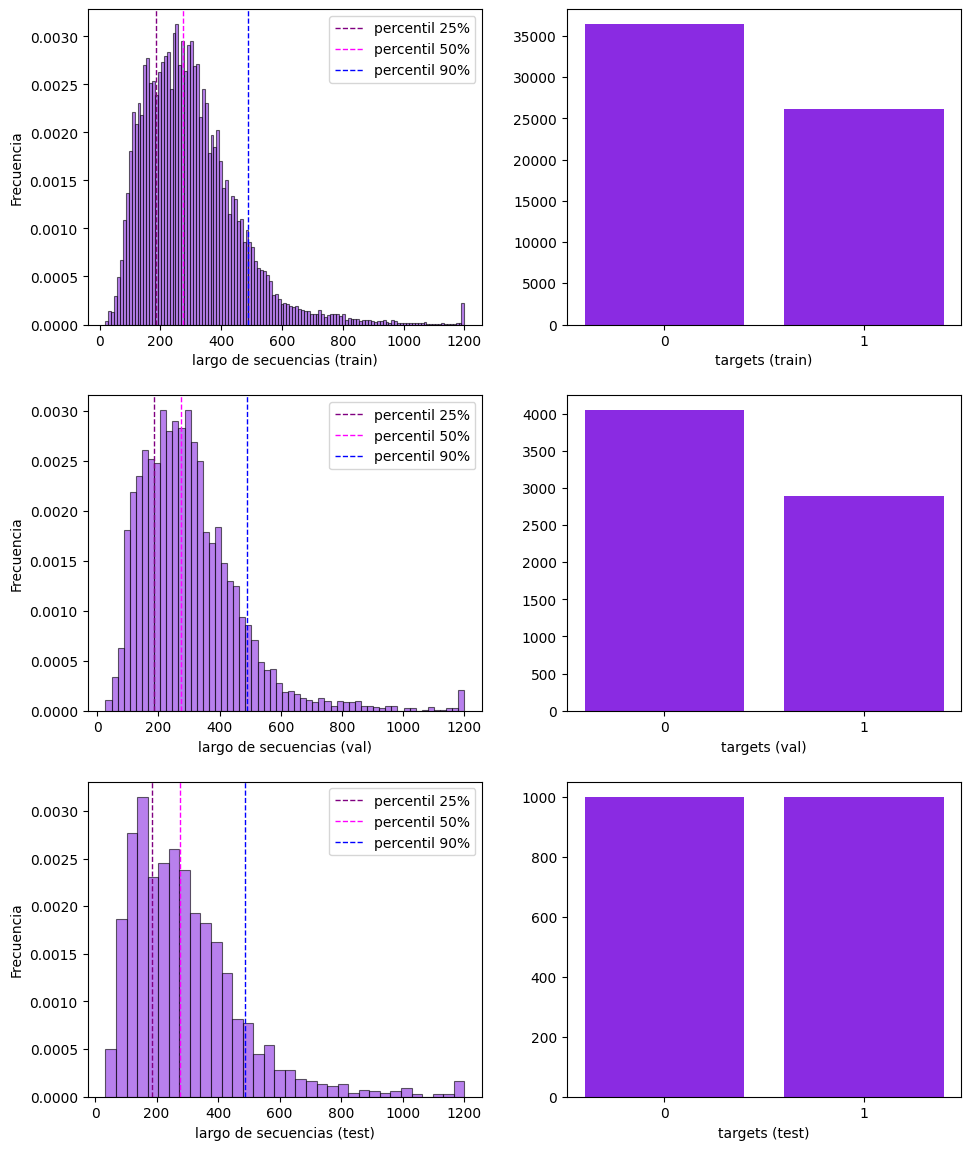
\includegraphics[scale=0.3]{/Users/ely/Documents/Maestria/proyecto_tecnologico/cimat2024-proyecto/Trabajo_final/latex/imagenes/output.png}
		\caption{Sequence length distributions of the training, validation and test sets. The 25th, 50th, and 90th percentiles of sequence lengths for the training, validation, and test sets are marked by dashed lines in the histograms.}
   \end{center} 
\end{figure}



Figure \ref{500amino} shows the distribution of the three subsets after taking all the protein sequences above 500 amino acids; as we can see, the binary labels still show balanced distributions.


Given that 90$\%$ of the sequences in the dataset are below 500 amino acids in length, we decided to limit the training to this subset. This decision was driven by practical considerations related to computational resources. Training on the original dataset with the full range of sequence lengths would require significant memory, potentially leading to inefficiencies and difficulties in model training. 


\begin{figure} [H]
	\begin{center}
		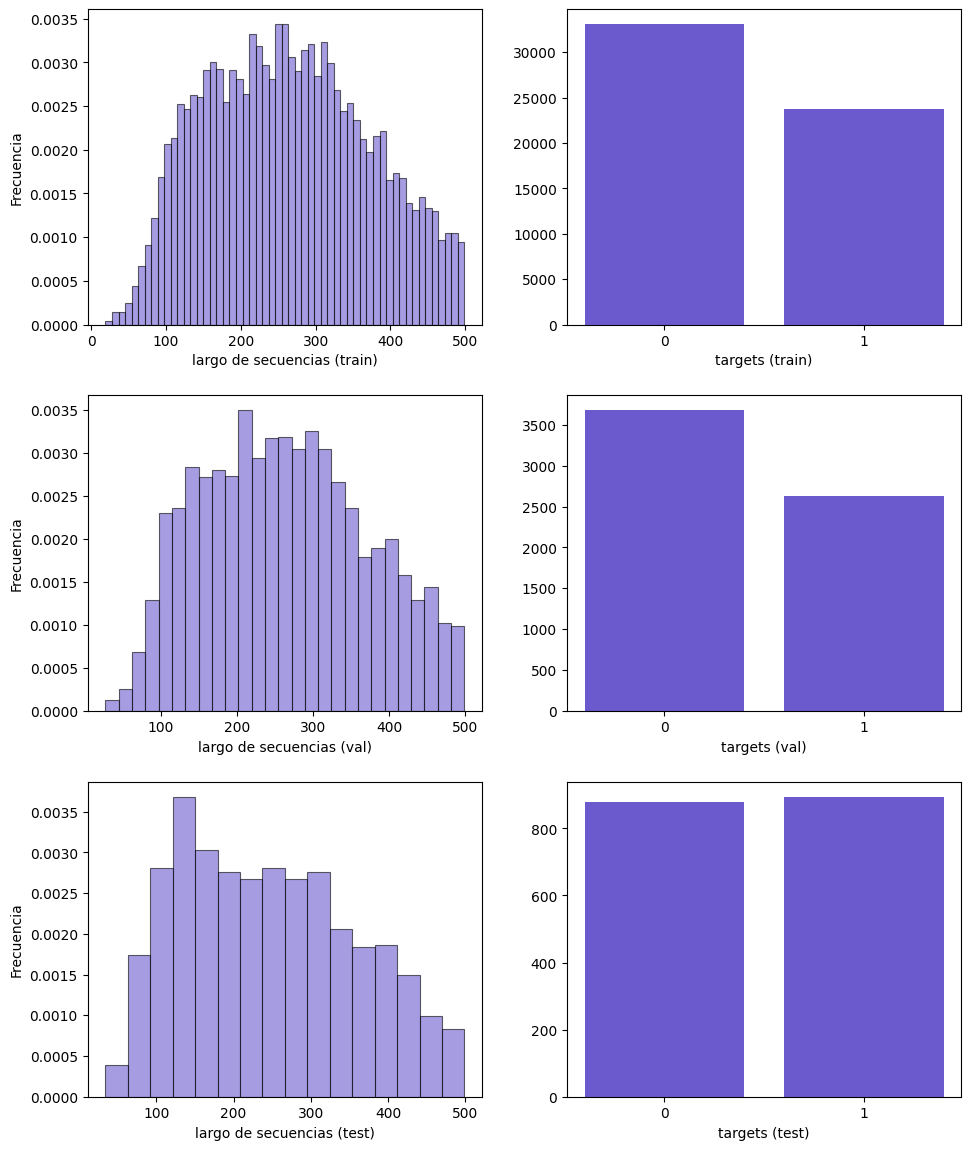
\includegraphics[scale=0.3]{/Users/ely/Documents/Maestria/proyecto_tecnologico/cimat2024-proyecto/Trabajo_final/latex/imagenes/output2.png}
		\caption{Sequence length distributions of the training, validation and test sets after taking all the sequences above 500 amino acids.}
      \label{500amino}
   \end{center} 
\end{figure}





\subsection*{Fluorescence}
For the fluorescence prediction task, we utilized a modified version of the PeptideBERT model. The following describes the architecture and configuration of the model used:


\begin{itemize}
   \item Vocab Size: 25
\item Hidden Size: 512
\item Num Hidden Layers: 16
\item Num Attention Heads: 16
\item Hidden Dropout Prob: 0.15
\item Max Position Embeddings: 256
\item Regression:  a fully connected layer that maintains the hidden size of 512, followed by a ReLU activation function to introduce non-linearity. To prevent overfitting, a dropout layer with a dropout probability of 0.15 is included, and the final linear layer outputs a single continuous value for the regression task.
\end{itemize}

For the fluorescence prediction task, we used the fluorescence dataset from the PEER benchmark, which is also accessible through the TorchDrug library. This dataset is used to predict the fitness of green fluorescent protein mutants. The target is the logarithm of fluorescence intensity annotated by Sarkisyan et al. The dataset splits are from TAPE \cite{TAPE}

The histogram above shows the distribution of sequence lengths in the entire dataset. All sequences are of approximately the same length, around 236 to 237 amino acids. 
The second histogram illustrates the distribution of fluorescence values (labels) in the dataset. The values range from approximately 1.5 to 4.0 on the logarithmic scale.

\begin{figure} [H]
	\begin{center}
		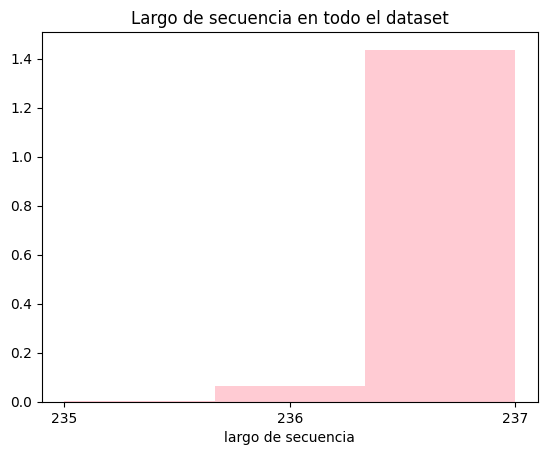
\includegraphics[scale=0.45]{/Users/ely/Documents/Maestria/proyecto_tecnologico/cimat2024-proyecto/Trabajo_final/latex/imagenes/output3.png}
		\caption{Sequence length distribution of the entire dataset.}
   \end{center} 
\end{figure}


\begin{figure} [H]
	\begin{center}
		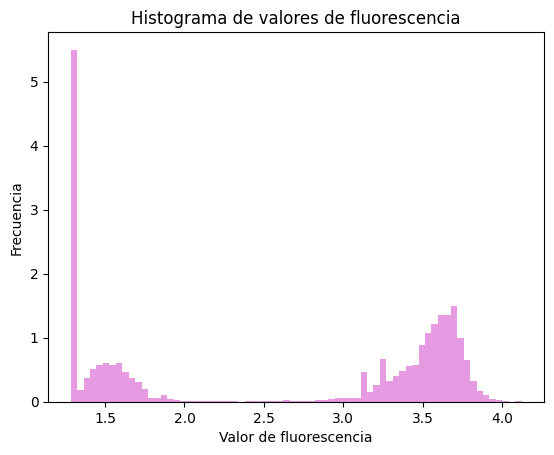
\includegraphics[scale=0.45]{/Users/ely/Documents/Maestria/proyecto_tecnologico/cimat2024-proyecto/Trabajo_final/latex/imagenes/output4.png}
		\caption{Label distribution of the entire dataset.} 
   \end{center} 
\end{figure}



\section{Results}

\subsection*{Solubility}
In the solubility prediction task, we evaluated the performance of our model using the modified PeptideBERT architecture. The classification report for the test set shows the following metrics: 


\begin{figure} [H]
	\begin{center}
		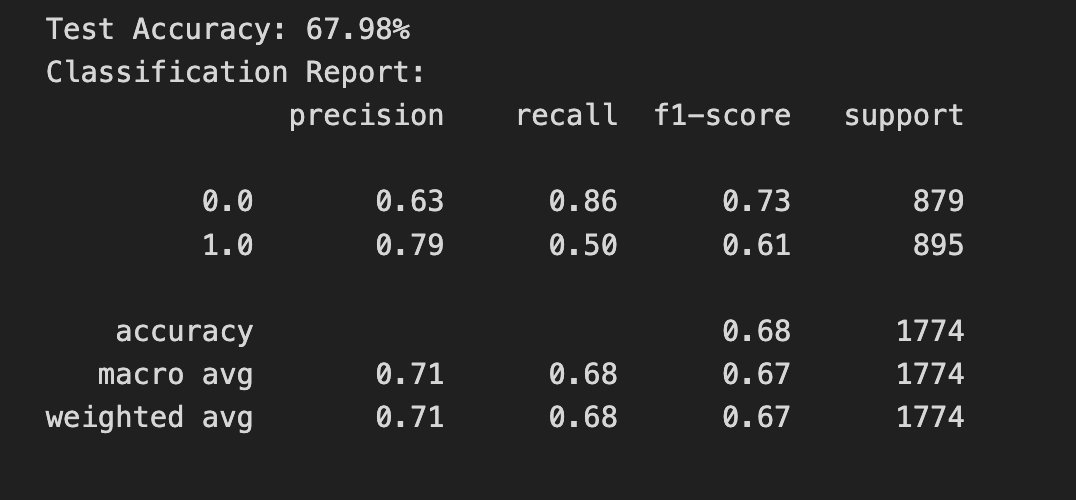
\includegraphics[scale=0.42]{/Users/ely/Documents/Maestria/proyecto_tecnologico/cimat2024-proyecto/Trabajo_final/latex/imagenes/solubility_results.png}
		\caption{Classification report for the test set in solubility task}
   \end{center} 
\end{figure}


The ProtBERT model in the PEER benchmark achieves a slightly higher accuracy of 68.15$\%$, but it uses the complete dataset, including sequences up to 1200 amino acids, and is trained for 50 epochs. 

Despite the differences in dataset size, training epochs, and model configuration, this model demonstrates competitive performance. The choice to limit sequence length to 512 amino acids was made to optimize memory usage. This decision, while reducing the overall dataset size, still allowed us to achieve a high level of accuracy close to that of the state-of-the-art models reported in the PEER benchmark.

\subsection*{Fluorescence}


In the fluorescence prediction task, we evaluated the performance of our model using the modified PeptideBERT architecture. The test Spearman's rank correlation coefficient was 0.23, which is relatively low. This outcome can be attributed to several factors, including the dataset's inherent nature, the model's inadequacy for this specific task, and the limited number of training epochs (30).

\begin{figure} [H]
	\begin{center}
		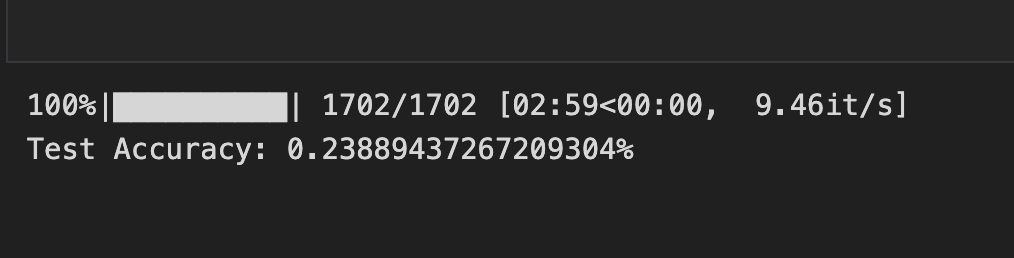
\includegraphics[scale=0.42]{/Users/ely/Documents/Maestria/proyecto_tecnologico/cimat2024-proyecto/Trabajo_final/latex/imagenes/fluoresensce_results.png}
		\caption{Test sSpearman's for the test set in fluorescence task}
   \end{center} 
\end{figure}

The best results reported in the PEER benchmark were achieved using a shallow CNN model, which obtained a Spearman's $\rho$ of 0.69. The PEER benchmark also includes models trained for a more extended period, allowing them to better capture the complex relationships within the data. 


\onecolumngrid

\section{Conclusion}
The modified PeptideBERT model demonstrated competitive performance in solubility prediction but is limited by computational resources. For fluorescence prediction, the low performance suggests exploring alternative models and extending the training epochs to capture the complex relationships in the data better.


Future work could consider architectures like the shallow CNN used in PEER, increasing training epochs and applying data augmentation strategies to improve model performance in predicting protein properties.

\onecolumngrid

\bibliographystyle{apsrev4-2}
\bibliography{references}




%%%%%%%%%%%%%%%%%%%%%%%%%%%%%%%%%%%%%%%%%%%%%%%%%%%%%%%%%%%%%%%%%%%%%%%%%%%%
%%%%%%%%%%%%%%%%%%%%%%%%%%%%%%%%%%%%%%%%%%%%%%%%%%%#5EJEMPLOS%%%%%%%%%%%%%
%%%%%%%%%%%%%%%%%%%%%%%%%%%%%%%%%%%%%%%%%%%%%%%%%%%%%%%%%%%%%%%%%%%%%%%%%%%%


%%%%%%%%%%%%%%%%%%%%%%%%%%%%%%%%%%%%%%%%%%%%%%%%%%%%%%%%%%%%%%%%%%%%%%%%%%%%
%%%%%%%%%%%%%%%%%%%%%%%%%%%%%%%%%%%%%%%%%%%%%%%%%%%%%%%%%%%%%%%%%%%%%%%%%%%%
%%%%%%%%%%%%%%%%%%%%%%%%%%%%%%%%%%%%%%%%%%%%%%%%%%%%%%%%%%%%%%%%%%%%%%%%%%%%

%%%%%%%%%%%%%%%%%%%%%%%%%%%%%%%%%%%%%%%%%%%%%%%%%%%%%%%%%%%%%%%%%%%%%%%%%%%%
%%%%%%%%%%%%%%%%%%%%%%%%%%%%%%%%%%%%%%%%%%%%%%%%%%%%%%%%%%%%%%%%%%%%%%%%%%%%
%%%%%%%%%%%%%%%%%%%%%%%%%%%%%%%%%%%%%%%%%%%%%%%%%%%%%%%%%%%%%%%%%%%%%%%%%%%%
%%%%%%%%%%%%%%%%%%%%%%%%%%%%%%%%%%%%%%%%%%%%%%%%%%%%%%%%%%%%%%%%%%%%%%%%%%%%



%%%%%%%%%%%%%%%%%%%%%%%%%%%%%%%%%%%%%%%%%%%%%%%%%%%%%%%%%%%%%%%%%%%%%%%%%%%%
%%%%%%%%%%%%%%%%%%%%%%%%%%%%%%%%%%%%%%%%%%%%%%%%%%%#6BIBLIOGRAFÍA%%%%%%%%%%%%%
%%%%%%%%%%%%%%%%%%%%%%%%%%%%%%%%%%%%%%%%%%%%%%%%%%%%%%%%%%%%%%%%%%%%%%%%%%%%


\end{document}


